\chapter{Models of Computation}

\section{PRAM}
\begin{paracol}{2}

   Idealized Shared-Memory platform with no caching, no NUMA organization, no synchronization overhead. The PRAM model is a theoretical model that is used to analyze the performance of parallel algorithms. It is a shared-memory model, where all processors can access all memory locations. The PRAM model is a simplification of the real world, and it is used to analyze the performance of parallel algorithms.
   \switchcolumn

   \begin{figure}[htbp]
      \centering
      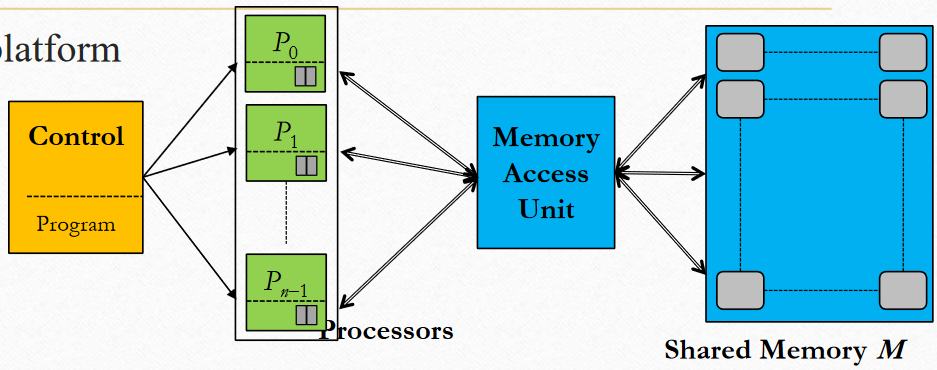
\includegraphics{images/07/pram.png}
      \caption{PRAM Model}
      \label{fig:07/pram}
   \end{figure}
   
\end{paracol}

There exist also variations of the PRAM model, such as the EREW (Exclusive Read Exclusive Write), CREW (Concurrent Read Exclusive Write), CRCW (Concurrent Read Concurrent Write), and ERCW (Exclusive Read Concurrent Write).

\section{Prefix Computation}

Given a binary associative operation $\circ$ on the set X: 
\begin{definition}
   [associative operation]
   \begin{equation}
      (x_1 \circ x_2) \circ x_3 = x_1 \circ (x_2 \circ x_3)
   \end{equation}
\end{definition}

\note{Examples are sum, product, max, min, string concat, boolean \texttt{and/or} etc.}

The prefix computation of a sequence $x_1, x_2, \ldots, x_n$ is the sequence $s_1, s_2, \ldots, s_n$ where:
\begin{abstract}
   \begin{align}
      s_0 = x_0 \\
      s_1 = x_0 \circ x_1 \\
      \ldots \\
      s_i = x_0 \circ x_1 \circ \ldots \circ x_{i} \quad i=0,\ldots,n-1\\
      s_i = s_{i-1} \circ x_i \quad i=1,\ldots,n-1\\
      s_n = x_1 \circ x_2 \circ \ldots \circ x_{n-1} \quad \text{\textred{Questo non mi torna molto}}
   \end{align}
\end{abstract}

\begin{definition}
   [Prefix computation]
   Obtaining $S = {s_0, s_1, \ldots, s_n}$ from $X = {x_0, x_1, \ldots, x_n}$ is called prefix computation.
\end{definition}

\subsection{Parallel Prefix Computation on PRAM}
Consider $\circ = +$ and a PRAM model with $n$ processors. The following algorithm computes the prefix sum of an array $A[0 \ldots n-1]$ in $O(nlog n)$ time using $n$ processors..
\begin{lstlisting}
   for (j = 0; j<n; j++) do_in_parallel   // each processor j
      reg_j = A[j];                       // copies one value to a local register
   for (i = 0; i<ceil(log(n)); i++) do    // sequential outer loop
      for (j = pow(2, i); j<n; j++) do_in_parallel // each proc. j
         reg_j += A[j - pow(2, i)];       // performs computation
         A[j] = reg_j;                    // writes result to shared memory
   }
\end{lstlisting}

$O(nlog n)$ is \textbf{not optimal}, we want to reach $O(n)$.
How can we do that?
\subsubsection{Approach 1}

Let's use $p = n/logn$ processors and apply the following algorithm:
\begin{enumerate}
   \item Partition the $n$ input values into chunks of size $log(n)$. Each processor computes local prefix sums of the values in one chunk in parallel (takes time $O(log(n))$).
   \item Perform the old non-cost-optimal prefix sum algorithm on the $n log(n)$ partial results (takes time $O(log(n/ log(n)))$).
   \item Each processor adds the value computed in step 2 by its left neighbor to all values of its chunk(takes time $O(log(n))$)
   \item[] Hence, the algorithm is \textit{cost-optimal}, since we get that
   \begin{equation}
      C(n) = T(n,p)\times p = O(log(n))\times \frac{n}{log(n)} = O(n)
   \end{equation}
 \end{enumerate}

\subsubsection{Approach 2}

ASsume you have a one-dimensional array A where most entries are zero.
We can represent the array in a more memory-efficient way by only storing the values of the non-zero entries (in \texttt{V}) and their corresponding coordinates (in \texttt{C}).

\begin{paracol}{2}
   
   
   We generate a temporary array ($tmp$) with $tmp[i] = 1$ if $A[i] != 0$ and $tmp[i] = 0$ otherwise. We then perform a parallel prefix summation on $tmp$. For each non-zero element of $A$, the respective value stored in $tmp$ now contains the destination address for that element in \texttt{V} .
   
   Then, we write the non-zero elements of $A$ to \texttt{V} using the addresses generated by the parallel prefix summation.
   The respective coordinates can be written to $C$ in a similar way.
   
   \switchcolumn

   \begin{figure}[htbp]
      \centering
      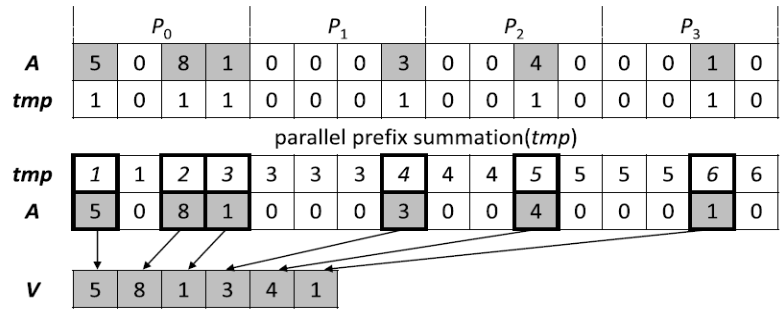
\includegraphics{images/07/sparsearray.png}
      \caption{Sparse Array Computation}
      \label{fig:07/sparsearray}
   \end{figure}

\end{paracol}

\section{Bulk Synchronous Parallel (BSP) Model}
This is more than a theoretical model, it is closer to reality than the PRAM model. It was proposed as a unified framework for the design, analysis, and programming of general-purpose parallel systems.

{It consists of three parts:\ns
\begin{itemize}
	\item A collection of processor-memory components
	\item A communication network that can deliver point-to-point messages among processors. It is a black box, no assumptions are made about its internal functioning.
	\item A facility for global synchronization (barrier) of all processors
\end{itemize}}

\newpage
\begin{paracol}{2}
   \begin{figure}[htbp]
      \centering
      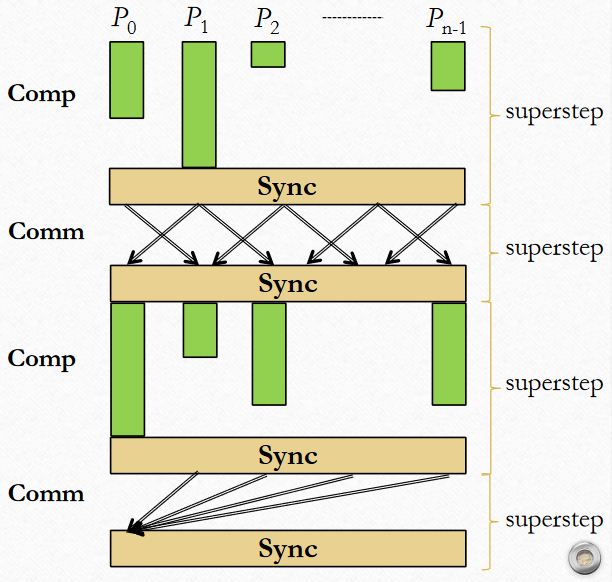
\includegraphics{images/07/bsp.png}
      \caption{Bulk Synchronous Parallel Model}
      \label{fig:07/bsp}
   \end{figure}
   
   \switchcolumn
   A BSP algorithm consists of a sequence of \textbf{supersteps}, which consist of
   \begin{itemize}
   	\item a number of computation or communication steps or both
   	\item called mixed superstep in case both are executed
   	\item a\textit{ global barrier} synchronization (bulk synchronization)
   \end{itemize}

   A \textbf{\textit{computation} superstep} consists of many small steps executing operations (e.g., floating point operations), while a \textbf{\textit{communication} superstep} consists of many basic communication operations (e.g., a data word transferring).

   A communication step hence is means transferring data from a memory to another

\end{paracol}

An h-relation is a communication superstep in which every processors sends and receives at most h
data words.
It is the maximum between the data words sent and received by a processor in a communication superstep.

\framedt{h-relations}{
   The cost of an h-relation is $T(h) = g * h + l$
   where:
   % • 𝑔 (gap) is the time per data word and 𝑙 (latency) is the global synchronization time


}

% The cost of a computation superstep is 𝑇𝑐𝑜𝑚𝑝 𝑤 = 𝑤 + 𝑙
% The cost of a mixed superstep (i.e., a superstep containing both computation and communication) is
% 𝑇𝑐𝑜𝑚𝑝 𝑤 = 𝑤 + ℎ ∙ 𝑔 + 𝑙

in general, the cost of a BSP algorithm is the sum of the costs of all supersteps.
\begin{equation}
   a + b * g + c * l
\end{equation}

\begin{figure}[htbp]
   \centering
   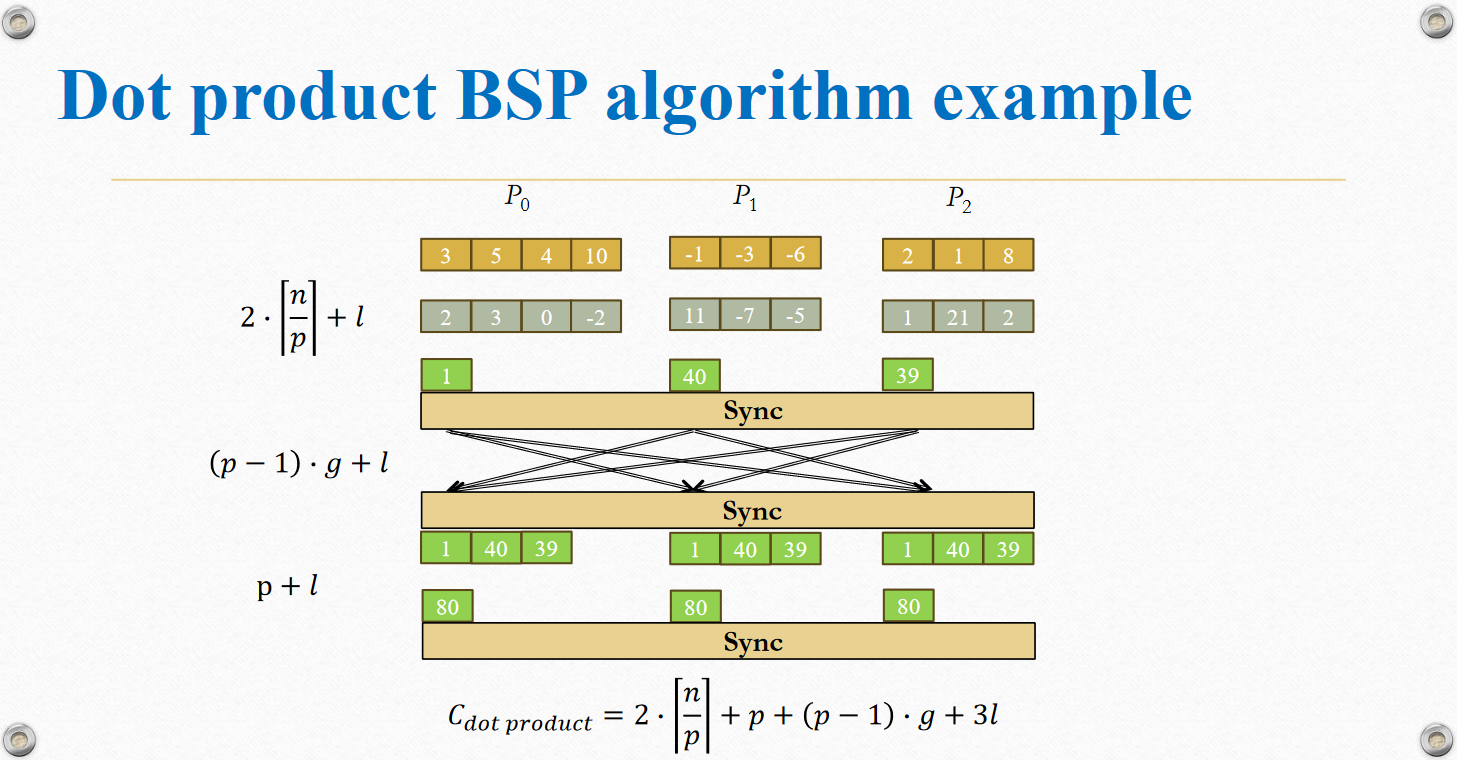
\includegraphics{images/07/bsp_example.png}
   \caption{BSP algorithm example}
   \label{fig:07/bsp_example}
\end{figure}

Recall that BSP is SPMD (Single Program Multiple Data) model, meaning that all processors execute the same program, but on different data.

\section{Work-Span Model}
The Work-Span model (also called Work-Depth) model is another classic performance model. It provides more strict bounds than those offered by the Amdahl's and Gustafson's laws.

The program's tasks form a DAG (Directed Acyclic Graph; a \textbf{task} is a unit of work, i.e., arbitrary sequential code, that can be executed in parallel (using threads or processes) with other program's tasks.

A given graph’s task is ready to run iff all its predecessors in the graph have been completed.
Hence, the edges represent a \textbf{data dependency} between tasks, i.e. the output of a task is the input of another task.

\note{
Let’s assume:
\begin{itemize}
	\item p identical processors, each executing one ready task at a time
	\item The task scheduling is greedy, i.e., whenever there is a ready task (and an available processor), the task is executed immediately
\end{itemize}
}

\begin{paracol}{2}
   \begin{figure}[htbp]
      \centering
      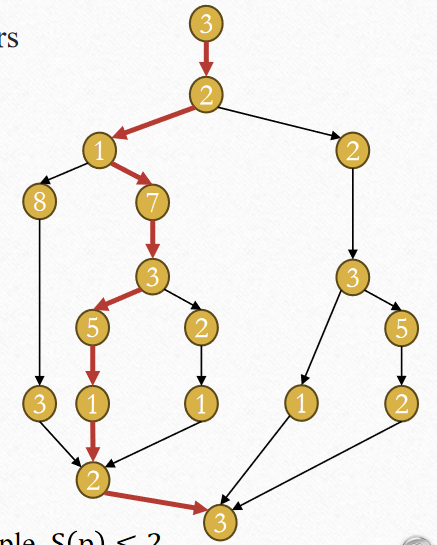
\includegraphics{images/07/ws.png}
      \caption{Work-Span Model}
      \label{fig:07/ws}
   \end{figure}
   
   \switchcolumn
\begin{itemize}
   \item $T_p$ is the time when executing with a greedy scheduler with $p$ processors
   \item $T_1$ is called \textit{work}
   \item $T_{\infty}$ is called \textit{span}, or \textit{critical path}
   \item In the example on the right we have $T_1 = 54$ and $T_{\infty} = 27$
   \item Let's consider the speedup to derive interesting bounds:
   \begin{align}
      S(p) = \frac{T_1}{T_p} \leq \frac{T_1}{\frac{T_1}{T_p}} = p \quad \textit{i.e. it is not possible to have superlinear speedup.}\\
      S(p) = \frac{T_1}{T_p} \leq \frac{T_1}{T_{\infty}} \leq p
   \end{align}
\end{itemize}
\end{paracol}

\section{Brent's Theorem}

\begin{itemize}
	\item Assume a parallel computer whose processors can perform a task in unit time with greedy scheduling of
tasks
	\item Assume that the computer has enough processors to exploit the maximum concurrency in an algorithm
containing $T_1$ tasks such that it completes in $T_{\infty}$ time steps.
	\item At each level $i$ of the DAG, there are $m_i$ tasks. We may use $m_i$ processors to compute all results in $O(1)$.
\end{itemize}
Brent's theorem states that a similar computer with fewer processors $p$ can execute the algorithm with the
following upper time limit on $T_p$:
\begin{equation}
   T_p \leq \frac{T_1 - T_{\infty}}{p} + T_{\infty}
\end{equation}

\subsection{Implications}
If $T_{\infty} \ll T_1$, then $T_1 - T_{\infty} \approx T_1$, therefore 
\begin{equation}
   T_p \leq \frac{T_1}{p} + T_{\infty} \quad \textit{if } T_{\infty} \ll T_1
\end{equation}

When designing a parallel algorithm, focus on reducing the span, because the span is the fundamental asymptotic limit on scalability. Increase the work only if it enables a drastic decrease in span.\\
Overall we have:

\begin{equation}
   \frac{T_1}{p} \leq T_p \leq \frac{T_1}{p} + T_{\infty}
\end{equation}

Additionally, it can be proved that
\begin{equation}
   S(p) = \frac{T_1}{T_p} \approx p \textit{ if } \frac{T_1}{T_{\infty}} \gg p
\end{equation}